%-----------------------------------------------------------------------------
%
%               Template for sigplanconf LaTeX Class
%
% Name:         sigplanconf-template.tex
%
% Purpose:      A template for sigplanconf.cls, which is a LaTeX 2e class
%               file for SIGPLAN conference proceedings.
%
% Guide:        Refer to "Author's Guide to the ACM SIGPLAN Class,"
%               sigplanconf-guide.pdf
%
% Author:       Paul C. Anagnostopoulos
%               Windfall Software
%               978 371-2316
%               paul@windfall.com
%
% Created:      15 February 2005
%
%-----------------------------------------------------------------------------


\documentclass{sigplanconf}

% The following \documentclass options may be useful:

% preprint      % Remove this option only once the paper is in final form.
% 10pt          To set in 10-point type instead of 9-point.
% 11pt          To set in 11-point type instead of 9-point.
% authoryear    To obtain author/year citation style instead of numeric.

\usepackage{amsmath}
\usepackage{natbib}
\usepackage{graphicx}
\usepackage{wrapfig}


\begin{document}

\special{papersize=8.5in,11in}
\setlength{\pdfpageheight}{\paperheight}
\setlength{\pdfpagewidth}{\paperwidth}

\conferenceinfo{CONF 'yy}{Month d--d, 20yy, City, ST, Country} 
\copyrightyear{20yy} 
\copyrightdata{978-1-nnnn-nnnn-n/yy/mm} 
\doi{nnnnnnn.nnnnnnn}

% Uncomment one of the following two, if you are not going for the 
% traditional copyright transfer agreement.

%\exclusivelicense                % ACM gets exclusive license to publish, 
                                  % you retain copyright

\permissiontopublish             % ACM gets nonexclusive license to publish
                                  % (paid open-access papers, 
                                  % short abstracts)

\titlebanner{banner above paper title}        % These are ignored unless
\preprintfooter{short description of paper}   % 'preprint' option specified.
\newcommand{\pname}{ErrorView}

\title{\pname{}}
\subtitle{Edit all touch points of a change simultaneously}

\authorinfo{Josh Terrell}
           {North Carolina State University (Affiliation..is this right?)}
           {jmterrel@calpoly.edu}
% \authorinfo{Name2\and Name3}
%            {Affiliation2/3}
%            {Email2/3}

\maketitle

\begin{abstract}
Some developers do not trust refactoring tools to refactor correctly. Without
using refactoring tools, refactoring can take longer and result in more bugs.
Developers don't have
to trust automated refactoring tools to take advantage of some productive
features that refactoring tools offer.
Using \pname{}, developers can refactor more quickly, with higher
quality, and without needing to trust automated refactoring tools.
% problem. why propblem is problem. startling sentence (make claim). implication.
\end{abstract}

\category{not sure what to put here..CR-number}{subcategory}{third-level}

% general terms are not compulsory anymore, 
% you may leave them out
% \terms
% term1, term2

\keywords
refactoring, tool, trust

\section{Introduction}
Research shows that software developers don't use automatic software
refactoring tools as often as the tools may be useful \cite{how-refactor}.
\textit{Awareness}\footnote{In this paper I refer to \textit{awareness} as both
the concepts \textit{awareness} (knowing of a tool) and \textit{opportunity}
(realizing that now is a good
time to use a tool) from \cite{how-refactor}} of refactoring tools and
\textit{trust} in the tools have
been observed to be two reasons for why developers don't use these tools
often \cite{how-refactor, say-refactor}.

Among other reasons, two reasons why developers lacking awareness of
automated refactoring tools don't use the tools is that they don't know that a
tool exists or don't realize they
are at a good place to use a tool until it is too late \cite{how-refactor}.

Developers who don't trust automated refactoring
tools know about the tools, but they don't trust the tool to refactor code
correctly. Some worry that refactoring tools may introduce bugs; others
are concerned with the readability and design of code output by the
tools \cite{say-refactor}.
Rather than using the tool, the developers opt-in for a manual refactor.

\pname{} aids developers who perform
refactorings but who don't trust refactoring tools. \pname{} does so by allowing
developers to simultaneously view and edit a refactoring's touch points
(areas of code changed in a refactoring). The goal of this tool is to support
developers' refactoring workflows without requiring them to use tools they don't
trust and interfaces they aren't familiar with.

\section{Related Work}
BeneFactor \cite{bene-factor} and WitchDoctor \cite{witch-doctor} are solutions
which both help increase the use of refactoring tools by addressing
developers' \textit{awareness} of refactoring tools.
BeneFactor and WitchDoctor help devlopers who don't know about a
refactoring tool or don't realize they are doing a refactoring until too late.
These tools detect when a refactoring is occuring and allow automatic completion
of the refactoring from the current snapshot of code
\cite{bene-factor, witch-doctor}.

GhostFactor takes a different apporach. GhostFactor tackles both the
\textit{awareness} and \textit{trust} reasons by (1) automatically detecting
when a developer has finished manually refactoring and (2) not interferring with
the developer's manual
refactorings, but instead validating that the developers have refactored
correctly \cite{ghost-factor}.

\section{Approach}
\pname{}'s approach is different than related tools in that it doesn't refactor
for you or even know how to refactor. Rather, \pname{} simply provides a
convinient and familiar interface for developers to perform refactorings in
thier own workflow.

Some developers use \textit{lean on the compiler} to refactor code
\cite{legacy-code}. Using \textit{lean on the compiler},
developers choosing to, for example, rename a method, first rename the method
declaration to something obscure. The result
is a bunch of errors scattered throughout the code. The developer subsequently
visits these errors, determines a better name for the method using the calling
contexts, renames all references to the method, and finally renames the
declaration.

\pname{} steps in where the developer visits all the errors scattered througout
the code. With this tool, developers can bring up quick fix for any error and
then choose to open all related errors in another tab.
\begin{center}
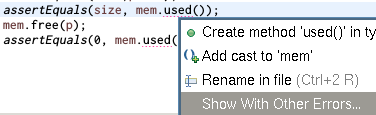
\includegraphics[width=0.35\textwidth]{quick-fix.png}
\end{center}

In the example, the developer wishes to rename the method
\textit{getValidMoves}, so he renames
it to something obscure. He then brings up the quick fix menu of the method
itself (Ctrl+1) or any of the newly created errors and selects
"Show With Other Errors..."

ErrorView subsequently displays a window containing a collection of
editors---each having
one of the related errors in focus. This multiple-editor window allows the
developer to simultaneously view the error
contexts to determine a more suitable method name. Then the developer may make
the desired renaming changes without needing to manually iterate through the
process of opening a new window for each error.
\begin{center}
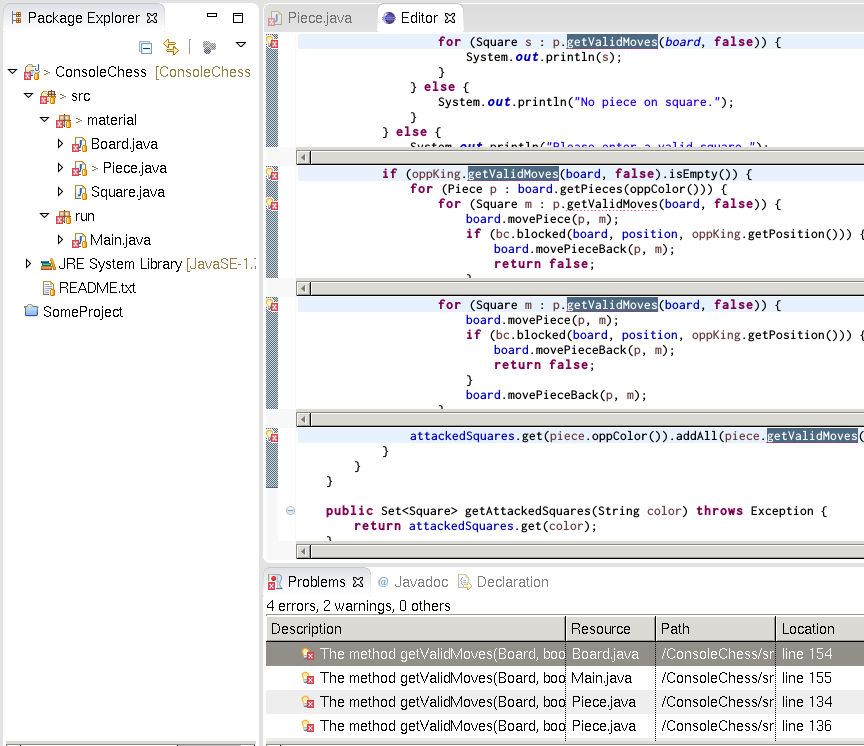
\includegraphics[width=0.50\textwidth]{multiple-editors.png}
\end{center}

The image shows each of the four related errors open and shown in their own
editor. A developer may now easily and quickly see all the contexts together,
choose an appropriate name, and complete the renaming of the method.

\section{Results}
Results, results, results, results. Results, results, results.
Results, results, results, results. Results, results, results.
Results, results, results, results. Results, results, results.
Results, results, results, results. Results, results, results.
Results, results, results, results. Results, results, results.
Results, results, results, results. Results, results, results.
Results, results, results, results. Results, results, results.
Results, results, results, results. Results, results, results.

Results, results, results, results. 
Results, results, results, results. Results, results, results.
Results, results, results, results. Results, results, results.
Results, results, results, results. Results, results, results.
\section{Future Work}
Future, future, future, future. Future, future, future, future.
Future, future, future, future. Future, future, future, future.
Future, future, future, future. Future, future, future, future.
Future, future, future, future. Future, future, future, future.

\appendix
% \section{Appendix Title}
% 
% This is the text of the appendix, if you need one.

\acks
thanks, thanks, thanks, thanks. thanks, thanks, thanks, thanks.
thanks, thanks, thanks, thanks. thanks, thanks, thanks, thanks.
thanks, thanks, thanks, thanks. thanks, thanks, thanks, thanks.

%Thank you Dr. Emerson Muphy-Hill for your guidance through writing my first
%research paper. Also a big thank you goes to the National Science Foundation
%which made this research opportunity and many like it possible.

% We recommend abbrvnat bibliography style.

\bibliographystyle{abbrvnat}

% The bibliography should be embedded for final submission.

\softraggedright
\bibliography{error-view}

\end{document}
